\section{General Design Decisions}

\subsection{Programming Language}

Choosing a programming language is one of the most essential aspect to take into account as it is the medium used to transform the system from design to implementation. However, choosing from over 250 different programming languages \citep{tiobe} can be tricky, which is why multiple views have to be evaluated before choosing a programming language. Four popular programming languages are considered for this project: Python, Java, R and  Javascript.\\

The first element to consider is the availability of third-party libraries used for implementing common machine learning methods, as well as data pre-processing, manipulation and visualisation techniques found in deep learning systems to avoid manually implementing them. The most popular libraries nowadays consist of Tensorflow (which is available in Python, R and Javascript) and PyTorch (which is available in Python). Additionally, Compute Unified Device Architecture (CUDA) support for GPU optimisations, CNN support and pre-trained models need to be included for the implementation of the desired deep learning breast cancer detection system, which are available in all libraries.\\

In terms of speed, compiled languages are quicker than interpreted languages. However, the main bottleneck in a deep learning system is the training phase of the model, which mainly relies on the library used rather than the language itself. Therefore, speed is not taken into account. Finally, of all the programming languages mentioned, Python is the favoured one in terms of personal preference, familiarity, and experience, especially when applied to machine learning implementations. Therefore, the wide support for machine learning libraries in Python, coupled with the personal preference for the language, make Python the obvious programming language candidate for this project.\\

For a complete review of the main pros and cons considered between when deciding between Python, Java, R and Javascript, refer to Appendix~\ref{sec:appendix-programming-languages-comparison}.

\subsection{Deep Learning Framework}

Due to the large nature of the datasets and complexity of the deep learning models to implement, powerful computing resources will be used in the form of Graphical Processing Units (GPU). A GeForce GTX 1060 6GB is provided by the School of Computer Science and remotely accessed via SSH to a lab machine equipped with the GPU in question running on CentOS.\\

To make use of the GPU's computing capabilities, deep learning frameworks with CUDA support (for parallel computing) should be used. The two most popular deep learning frameworks nowadays are Tensorflow coupled with Keras, and PyTorch. Tensorflow/Keras being relatively older than PyTorch, have got more online support, which is confirmed by the number of daily downloads Keras has compared to PyTorch (ten times more), as well as the number of mentions in academic papers (see figures  in Appendix~\ref{sec:appendix-keras_vs_pytorch})

\subsection{Interface}

A Command-Line Interface (CLI) is selected, allowing arguments and flags to be passed to execute different sections of the code. Arguments control the dataset to use, the CNN model, and the mode to run in (training or testing). Flags control the verbose mode to print more statements in the terminal for debugging purposed. The full set of instructions to run the code can be found in Appendix~\ref{ch:appendix-usage-instructions}.

%%%%%%%%%%%%%%%%%%%%%%%%%%%%%%%%%%%%%%%%%%%%%%%%%%%%%%%%%%%%%%%%%%%%
%%%%%%%%%%%%%%%%%%%%%%%%%%%%%%%%%%%%%%%%%%%%%%%%%%%%%%%%%%%%%%%%%%%%
%%%%%%%%%%%%%%%%%%%%%%%%%%%%%%%%%%%%%%%%%%%%%%%%%%%%%%%%%%%%%%%%%%%%

\section{Datasets}

An early design decision taken as a group consisted in which datasets to use. Two datasets, mini-MIAS and CBIS-DDSM, are used for this project as they have different characteristics.\\

From a clinical point of view, the mini-MIAS dataset is an interesting dataset as it contains the abnormal cases, like the ones found in the CBIS-DDSM dataset, and normal cases as well. resulting in three classes (normal, benign and malignant cases). Its smaller size makes it useful for initial prototyping, but has the downside of requiring image processing techniques such as data augmentation to generate enough data to feed into the deep learning model.\\

The CBIS-DDSM dataset was chosen over the DDSM dataset as it is an updated version of the older DDSM dataset, and is curated by a trained mammographer. Additionally, it uses uncompressed images in DICOM format rather than LJPEG format, which is deprecated nowadays, resulting in much better quality. Indeed, the large uncompressed format offered by DICOM means that the mammograms can be fed into the CNN with larger sizes, allowing the model to learn more low-level features. Despite the CBIS-DDSM dataset containing two different types of mammograms (calcification and masses), as well as two different views (CC and MLO), the mammograms in each case are treated as separate individual images due to the limited number of samples available.

%%%%%%%%%%%%%%%%%%%%%%%%%%%%%%%%%%%%%%%%%%%%%%%%%%%%%%%%%%%%%%%%%%%%
%%%%%%%%%%%%%%%%%%%%%%%%%%%%%%%%%%%%%%%%%%%%%%%%%%%%%%%%%%%%%%%%%%%%
%%%%%%%%%%%%%%%%%%%%%%%%%%%%%%%%%%%%%%%%%%%%%%%%%%%%%%%%%%%%%%%%%%%%

\section{Deep Learning Pipeline Design Considerations}

The deep learning pipeline implemented for the task of breast cancer detection can be broken down in four distinct phases condensed in Figure~\ref{fig:design-flowchart}:

\begin{itemize}
    \item Data pre-processing: loading one of the datasets in memory and processing them for the classification task (processing images and encoding labels).
    \item Model training: creating a CNN model and fitting the training data. Fine tuning carried out by testing various combinations of CNN models and hyperparameters.
    \item Result visualisation: Reporting the numerical predictions and plotting the results.
    \end{itemize}

\begin{figure}[ht]
\centerline{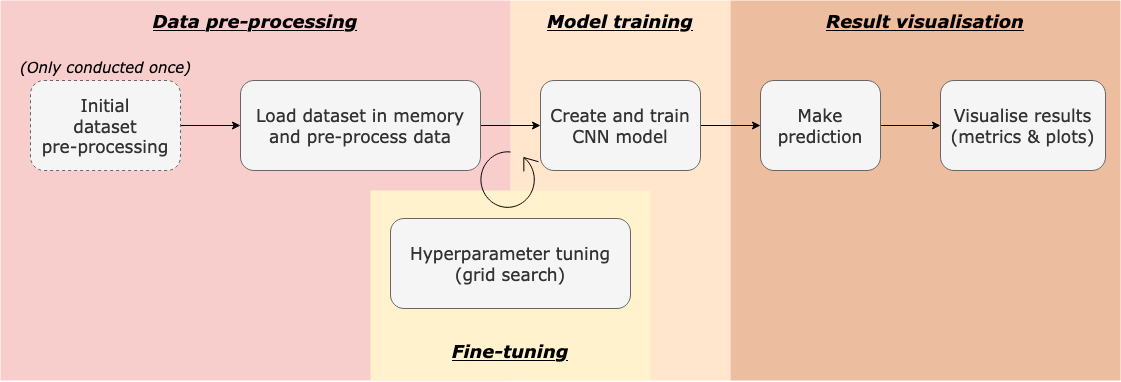
\includegraphics[width=1.1\textwidth]{Dissertation/figures/design/design flowchart.png}}
\caption{\label{fig:design-flowchart}High-level flowchart of the breast cancer detection deep learning pipeline to implement. Created using Draw.io.}
\end{figure}

%%%%%%%%%%%%%%%%%%%%

\subsection{Data pre-processing}

\subsubsection{Classification type}

Classification on the mini-MIAS dataset will be a multi-class problem as there are three possible classes (normal, benign and malignant), whereas classification on the CBIS-DDSM dataset will be a binary problem as it only contains abnormal classes (benign and malignant).

\subsubsection{Dataset balance}

As this is a classification task, it is essential to visualise the distribution of classes in the datasets to determine whether the data balance is skewed or not (whether some classes are much more frequent than other classes \citep{Geron2019}). The class distributions are plotted in Figure~\ref{fig:design-datasets-balance}.

\begin{figure}[h]
\centering
\begin{subfigure}{.5\textwidth}
  \centering
  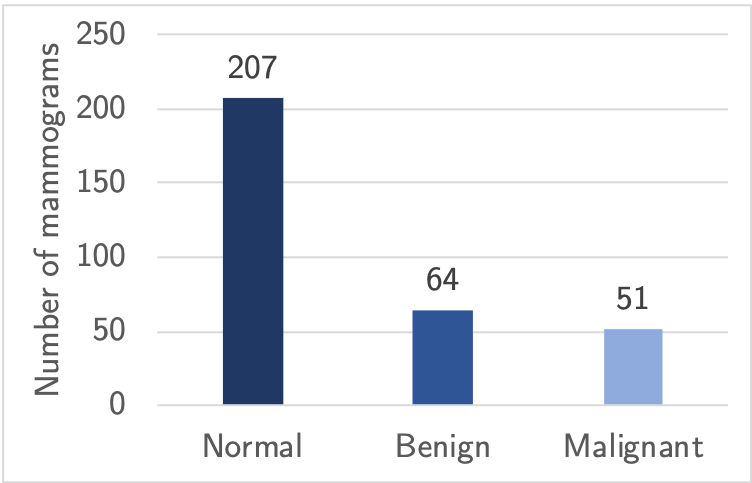
\includegraphics[width=0.94\textwidth]{Dissertation/figures/design/mini-mias-balance.png}
  \caption{mini-MIAS class distribution.}
  \label{fig:design-mini-mias-balance}
\end{subfigure}%
\begin{subfigure}{.5\textwidth}
  \centering
  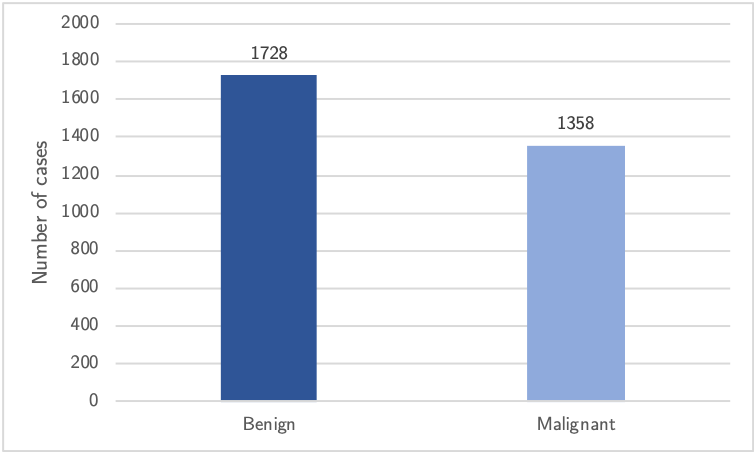
\includegraphics[width=\textwidth]{Dissertation/figures/design/cbis-ddsm-balance.png}
  \caption{CBIS-DDSM class distribution.}
  \label{fig:cbis-ddsm-balance}
\end{subfigure}
\caption{\label{fig:design-datasets-balance}Class distribution for the mini-MIAS and the CBIS-DDSM datasets. Histograms generated in Excel.}
\end{figure}

These bar charts reveal that the mini-MIAS dataset is heavily unbalanced, which must be taken into account to avoid training a biased CNN model. Potential solutions to counter this imbalance would be to either:
\begin{itemize}
    \item \textit{undersample} the dataset by dropping images altogether,
    \item \textit{oversample} the dataset, which can be achieved via data augmentation,
    \item include \textit{class weights} to give more importance to under-represented classes. 
    %https://datascience.stackexchange.com/questions/13490/how-to-set-class-weights-for-imbalanced-classes-in-keras 
    %https://www.tensorflow.org/tutorials/structured_data/imbalanced_data#class_weights
\end{itemize}

Undersampling the dataset can be considered as inefficient as it will diminish the number of samples the model could learn from. As the datasets are already very small (maximum of 10,239 images), undersampling would be a poor strategy as it may discard useful features that could be learned. Consequently, oversampling by creating new data resembling the original data is a viable solution as it was proven to increase accuracies (see Section~\ref{sec:litsurvey-data-augmentation}). Alternatively, a cheaper option in terms of computing power that does not require the dataset to be touched would be to add class weights, which will be cause the loss to become a weighted average giving more importance to less frequent classes.

\subsubsection{Data loading}

The mini-MIAS dataset is very small in size (339 Mb before pre-processing, 202 Mb after pre-processing), containing only 322 images. It can therefore be loaded into memory without any data loading optimisation techniques. However, the CBIS-DDSM dataset is much larger, containing 10,239 images that cover 163.6 Gb of disk space. The dataset therefore cannot be loaded in memory in a single import and needs to be loaded in batches to be fed into the CNN sequentially. % mention batches and caching

\subsubsection{Label encoding}

As the labels for each mammogram are in categorical string format, they must be encoded into a numerical format. One-hot encoding is therefore chosen as it suits the sparse representation of the data, which is made up of only two or three target categories, depending on the dataset being used. The one-hot encodings of the labels can be seen in Table~\ref{tab:label-encoding-example}.

\begin{table}[h]
\centering
\begin{tabular}{|c|c|}
\hline
\textbf{Categorical format} & \textbf{One-hot encoding} \\ \hline
\textit{Normal}             & 1 0 0            \\ \hline
\textit{Benign}             & 0 1 0            \\ \hline
\textit{Malignant}          & 0 0 1            \\ \hline
\end{tabular}
\caption{Conversion from string (categorical) format to one-hot (numerical) encoding.}
\label{tab:label-encoding-example}
\end{table}

%%%%%%%%%%%%%%%%%%%%

\subsection{Model training}

To complete:
\begin{itemize}
    \item Training/testing/validation split using stratified and shuffling splits (keep class balance and reorder images in directories).
    \item CNN models with pre-trained weights on ImageNet to avoid training from scratch. However, this  forces the input images to have the same size as the images in ImageNet it was trained on.
    \item Early stopping conditions.
    \item Describe process of using pre-trained weights on ImageNet, freezing this layers and training fully connected layers, then unfreezing the pre-trained model and and learning with at a slower learning rate.
\end{itemize}

%%%%%%%%%%%%%%%%%%%%

\subsection{Result visualisation}
\label{sec:design-results-visualisation}

These bar charts reveal that the mini-MIAS dataset is heavily unbalanced, which must be taken into account when analysing the classifiers' scores. Indeed, using an  evaluation metric such as accuracy would be misleading as it would not be representative of how well the classifier fitted the data. For instance, if a dumb classifier that always classified an image as ``normal'' was created, it would achieve 64.28\% accuracy on the mini-MIAS dataset. Therefore, other metrics such as confusion matrices, precision, recall and F1 scores could be used.\\

Different output metrics are chosen to assess how well the CNN learned the mammograms data and generalises to unseen cases. A combination of numerical metrics and visual metrics are used:

\begin{itemize}
    \item Numerical metrics:
    \begin{itemize}
        \item Overall accuracy
        \item Precision
        \item Recall
        \item F1 score
    \end{itemize}
    \item Visual metrics (plots):
    \begin{itemize}
        \item Evolution of training/validation accuracies and losses over the number of epochs
        \item Confusion matrices
        \begin{itemize}
            \item Classification counts
            \item Normalised (values between 0 and 1)
        \end{itemize}
        \item Receiver Operating Characteristic (ROC) curve
    \end{itemize}
\end{itemize}
